% concatenated from main.tex
\documentclass[11pt]{amsart}

\usepackage[margin=1in]{geometry}
\usepackage{amsmath,amssymb,amsthm,mathtools}
\usepackage{enumitem}
\usepackage{microtype}
\usepackage[hidelinks]{hyperref}
\usepackage{tikz}

\newtheorem{theorem}{Theorem}[section]
\newtheorem{proposition}[theorem]{Proposition}
\newtheorem{lemma}[theorem]{Lemma}
\newtheorem{corollary}[theorem]{Corollary}
\newtheorem{remark}[theorem]{Remark}
\newtheorem{definition}[theorem]{Definition}
\newtheorem{question}[theorem]{Question}

\newcommand{\Mbar}{\overline{\mathcal M}}
\newcommand{\Mbarzn}{\overline{\mathcal M}_{0,n}}
\newcommand{\Mbargn}{\overline{\mathcal M}_{g,n}}
\newcommand{\Mgn}{{\mathcal M}_{g,n}}
\newcommand{\Pn}{P_n}
\newcommand{\Fm}{F_m}
\newcommand{\RR}{\mathbb R}
\newcommand{\QQ}{\mathbb Q}
\newcommand{\dd}{\,d}
\newcommand{\ulc}{\operatorname{ULC}}


%\usepackage[notcite, notref]{showkeys}
\newcommand{\PP}{\mathbb{P}} 
\newcommand{\cM}{\mathcal{M}} 
\newcommand{\bcM}{\overline{\cM}}
\newcommand{\bt}{\tilde{b}}
\newcommand{\Pt}{\widetilde{P}}
\newcommand{\Ft}{\widetilde{F}}
\def\cM{\mathcal{M}}
\def\ZZ{\mathbb{Z}}
\def\CC{\mathbb{C}}
\def\LL{\mathbb{L}}
\def\lra{\longrightarrow}
\def\beq{\begin{equation}}
\def\eeq{\end{equation}}
\def\tF{\widetilde{F}}
\def\HH{\mathbb{H}}
\def\FF{\mathbb{F}}
\def\KV{\mathrm{K}(\mathbf{V}) }
\def\KVG{\mathrm{K}(\mathbf{V},G)}
\def\FM{\mathrm{FM}}

\usepackage{pgfplots}
\pgfplotsset{compat=1.18}

\title{Stratified motivic invariants and bivariate deformations of Poincar\'e polynomials}
\author{Gergely B\'erczi and Young-Hoon Kiem}
\date{}
\address{Department of Mathematics, Aarhus University, Ny Munkegade 118, 8000 Aarhus, Denmark}
\email{gergely.berczi@math.au.dk}
\address{School of Mathematics, Korea Institute for Advanced Study, 85 Hoegiro, Dongdaemun-gu, Seoul 02455, Korea}
\email{kiem@kias.re.kr}


\begin{document}
\begin{abstract}
    For a stratified variety $X$ and a motivic invariant $\HH$, we consider the stratified invariant which interpolates the invariant of $X$ and that of its interior $X^\circ$. Based on observations in moduli theory, we introduce the notion of an echelon tower of stratified varieties and then prove explicit inductive formulae for the stratified invariants of the moduli spaces $\Mbarzn$ of stable curves of genus $0$ and the Fulton-MacPherson varieties $Y[n]$ for any smooth projective variety $Y$. Using these, we show that the mysterious bivariate deformations of the even degree Poincar\'e polynomials of $\bcM_{0,n+1}$ and $\PP^1[n]$ in \cite{BercziKiem2026} are nothing but stratified virtual Poincar\'e polynomials.    
\end{abstract}

\maketitle

\section{Introduction}

Let $\HH$ denote a motivic invariant such as the Hodge-Deligne polynomial or the virtual Poincar\'e polynomial. Let $X$ be a quasi-projective variety of dimension $m$ over $\CC$ with a stratification 
$$X=X_0\supset X_1\supset \cdots \supset X_m\supset X_{m+1}=\emptyset$$
by closed subvarieties such that $X_j^\circ=X_j-X_{j+1}$ is smooth of codimension $j$ or empty for each $j$. Then we can consider the \emph{stratified motivic invariant}
\beq\label{i3} \FF_X(y)=\sum_{j=0}^m y^j\HH_{X_j^\circ}\eeq 
which refines the motivic invariant of $X$ since $\FF_X(1)=\HH_X$. 
The first question that we want to address in this paper is the following.

\begin{question}
    How can we compute the stratified motivic invariants?
\end{question}

Important spaces in moduli theory often admit natural stratifications and come in families which are closely connected. For example, the moduli spaces of stable curves $\Mbargn$ are stratified by the dual graphs and are connected by the forgetful morphisms $\pi_n:\bcM_{g,n+1}\to \Mbargn$. Likewise, the Fulton-MacPherson compactifications $Y[n]$ of the configuration spaces of $n$ ordered distinct points in a smooth projective variety $Y$ are stratified by the dual graphs and connected by the forgetful morphisms $\pi_n:Y[n+1]\to Y[n]$.
As the forgetful morphisms arise from contracting a rational component if necessary after deleting the last marked point, the number of irreducible components reduces at most by 1. 
We can codify these observations as follows.

\begin{definition} [Definition \ref{m19}]
    A sequence of stratified spaces $X[n]$ for $n\ge n_0$ together with morphisms $\pi_n:X[n+1]\to X[n]$ are said to form an \emph{echelon tower} if $\pi_n(X[n+1]_j^\circ)\subset X[n]_j^\circ\cup X[n]_{j-1}^\circ.$ We call the echelon tower \emph{solid} if the restrictions 
    $$\pi_{n,j,0}:X[n+1]_j^\circ\cap \pi_n^{-1}(X[n]_j^\circ)\lra X[n]_j^\circ, \ \ \ 
\pi_{n,j,1}:X[n+1]_j^\circ\cap \pi_n^{-1}(X[n]_{j-1}^\circ)\lra X[n]_{j-1}^\circ $$
    of $\pi_n$ are motivically locally trivial. 
\end{definition}
For a solid echelon tower, we can compute the stratified invariant $\FF_{X[n]}$ by an inductive formula. 

\begin{theorem} [Proposition \ref{m15} and Theorem \ref{m14}] \label{i1}
    The moduli spaces $\Mbarzn$ of stable curves of genus $0$ form a solid echelon tower and the stratified invariant $\FF_{\Mbarzn}(y)$ is uniquely determined by the inductive formula
    \beq\label{i5} \FF_{\bcM_{0,n+1}} = (ny-n+1+\LL)\FF_{\Mbarzn}+y(y+\LL-1)\,\partial_y\FF_{\Mbarzn}, \quad \FF_{\bcM_{0,3}}=1\eeq
where $\LL=\HH_\CC$.
\end{theorem}
This is an effective way of computing the stratified invariants because the formula does not involve a sum over graphs or a sum over the product of $\bcM_{0,k}$ for all $k< n$ or inverting a complicated power series.  
We can easily derive previously known formulae for the Poincar\'e polynomial of $\Mbarzn$ from \eqref{i5}. 

\begin{theorem}[Theorem \ref{f8}] \label{i2}
    The Fulton-MacPherson varieties $Y[n]$ for a smooth projective variety $Y$ form a solid echelon tower and $\FF_{Y[n]}$ is uniquely determined by 
    \[\FF_{Y[n+1]}=\left(\HH_Y-n+ny\HH_{\PP^{m-1}}\right)\FF_{Y[n]}+ y\left(y\HH_{\PP^{m-1}}+ ({\LL^m}-1)\right)\partial_y\FF_{Y[n]},\quad \FF_{Y[1]}=\HH_Y.\]
\end{theorem}
From this, by specializing to $y=1$, we can derive previously known formulae for the Poincar\'e polynomials of $Y[n]$ including Manin's formulae \cite[(4.22) and (4.24)]{Manin1999} by elementary calculus.

\medskip

In \cite{BercziKiem2026}, it was proved that the even degree Poincar\'e polynomial of $\Mbarzn$ defined by 
\beq\label{i7}
P^{even}_{n}(t)=\sum_it^i\dim H^{2i}(\bcM_{0,n})\quad \text{or}\quad P^{even}_{n}(t^2)=P_{\Mbarzn}(t)\eeq 
has only real roots and hence the even degree Betti numbers form an ultra-log-concave sequence. In fact, the proof was assisted by AI which introduced, seemingly out of nowhere, a bivariate polynomial $F_n(y,t)$ such that $F_n(1,t)$ coincides with $P^{even}_{n+1}(t)$.
Obviously, the real curve in $\RR^2$ defined by $F_n(y,t)=0$ meets the line $y=1$ at the real roots of $P^{even}_{n+1}(t)$. By induction, it was shown that for a fixed $t=0^-$, $F_n(y,t)$ has $n-2$ distinct roots in the interval $(0,1)$ while for a sufficiently negative fixed $t$, $F_n(y,t)$ has $n-2$ distinct roots in the interval $(1,\infty)$. Since the curve is smooth by the implicit function theorem, it follows from a Sturm-Liouville argument and a degree count that $P^{even}_{n+1}(t)$ has $n-2$ simple negative roots. The same was proved for the Fulton-MacPherson variety $\PP^1[n]$. 

\begin{center}
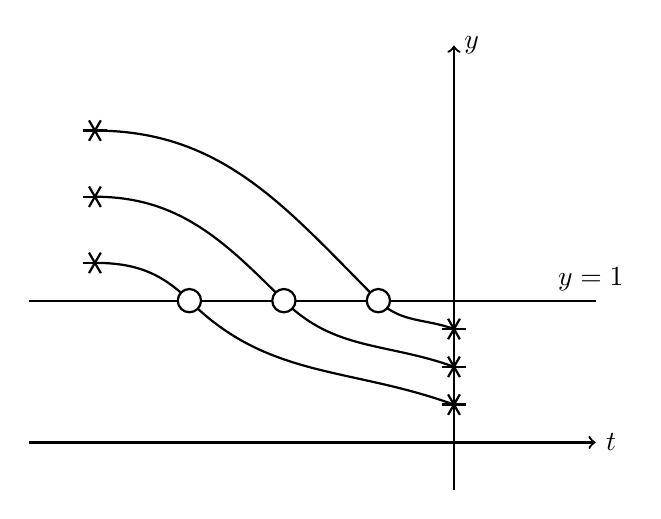
\begin{tikzpicture}[
    scale=1.2,
    dot/.style={circle, fill=black, inner sep=1.5pt},
    arrow/.style={->, thick, >=stealth}
]

\tikzset{
    asterisk/.pic={
        \draw[thick] (-0.15,0) -- (0.15,0);
        \draw[thick] (-0.075,-0.13) -- (0.075,0.13);
        \draw[thick] (-0.075,0.13) -- (0.075,-0.13);
    }
}

\draw[->, thick] (-4.5, 0) -- (1.5, 0) node[right] {$t$};
\draw[->, thick] (0, -0.5) -- (0, 4.2) node[right] {$y$};

\draw[thick] (-4.5, 1.5) -- (1.5, 1.5);
\node[above right] at (1, 1.5) {$y=1$};

\draw[thick] (-3.8, 3.3) to[out=0, in=135] (-0.8, 1.5) to[out=-45, in=160] (0, 1.2);
\draw[thick] (-3.8, 2.6) to[out=0, in=135] (-1.8, 1.5) to[out=-45, in=160] (0, 0.8);
\draw[thick] (-3.8, 1.9) to[out=0, in=135] (-2.8, 1.5) to[out=-45, in=160] (0, 0.4);

\pic at (-3.8, 3.3) {asterisk};
\pic at (-3.8, 2.6) {asterisk};
\pic at (-3.8, 1.9) {asterisk};

\pic at (0, 1.2) {asterisk};
\pic at (0, 0.8) {asterisk};
\pic at (0, 0.4) {asterisk};

\filldraw[fill=white, thick] (-0.8, 1.5) circle (3.5pt);
\filldraw[fill=white, thick] (-1.8, 1.5) circle (3.5pt);
\filldraw[fill=white, thick] (-2.8, 1.5) circle (3.5pt);

\end{tikzpicture}
\end{center}
\medskip

Although the proof of the real-rootedness of the even degree Poincar\'e polynomial $P^{even}_{n}(t)$ of $\Mbarzn$ is complete, the geometric meaning of the key ingredient $F_n(y,t)$ has remained a mystery. So it is reasonable to ask the following. 
\begin{question}\label{i4}
    Is there a natural geometric meaning of the bivariate deformation $F_n(y,t)$ (resp. $\widetilde{F}_n(y,t)$) of the even degree Poincar\'e polynomial of $\bcM_{0,n+1}$ (resp. $\PP^1[n]$) in \cite{BercziKiem2026}?
\end{question} 

As an application of Theorems \ref{i1} and \ref{i2}, we obtain the following answer to Question \ref{i4}.
\begin{corollary} [Corollary \ref{m17} and Corollary \ref{f21}]\label{i6}
    (1) The bivariate deformation $F_n(y,t^2)$ of the Poincar\'e polynomial of $\bcM_{0,n+1}$ coincides with $y\FF_{\bcM_{0,n+1}}(y,t)$ where 
    %$\FF$ denotes the stratified virtual Poincar\'e polynomial \eqref{i3} with 
    $\HH$ is the virtual Poincar\'e polynomial. 

    (2) The bivariate deformation $\widetilde{F}_n(y,t^2)$ of the Poincar\'e polynomial of $\PP^1[n]$ in \cite{BercziKiem2026} is precisely the stratified virtual Poincar\'e polynomial $\FF_{\PP^1[n]}(y,t)$.  
\end{corollary} 
The $t^2$ appears in Corollary \ref{i6} from 
$P^{even}_{n}(t^2)=P_{\Mbarzn}(t)$ and the same for $\PP^1[n]$.
%we are deleting the odd degree terms in the Poincar\'e polynomials to get the even degree Poincar\'e polynomials.  

\medskip

It will be interesting to see if the ideas in this paper and \cite{BercziKiem2026} extend to Chow rings of matroids and give us the real-rootedness of the Poincar\'e polynomials of loopless matroids. 




\bigskip

\section{Motivic invariants, stratified varieties and echelon towers}
In this section, we introduce the notions of motivic invariants, stratified varieties and echelon towers. 

\subsection{Motivic invariants of stratified varieties}
Let $\KV$ denote the Grothendieck ring of quasi-projective varieties over $\CC$. A \emph{motivic invariant} is a homomorphism 
$$\HH:\KV\lra R,\quad [X]\mapsto \HH_X$$
to an integral domain $R$ with unity such that $\HH_{[\mathrm{pt}]}=1$ and $\LL:=\HH_\CC$ invertible. 
In particular, we have 
\begin{enumerate}
    \item $\HH_X=\HH_Y+\HH_{X-Y}$ for a closed subvariety $Y\subset X$ and 
    \item $\HH_{X\times Z}=\HH_X \cdot \HH_Z$ for varieties $X$ and $Z$. 
\end{enumerate} 
As a consequence, if $X\to Y$ is a Zariski locally trivial morphism with fiber $Z$, we have $\HH_X=\HH_Y\cdot \HH_Z$. 
In what follows, we will use suitable extensions of the ring $R$, such as its field of fractions, whenever necessary.

%\medskip

%\noindent \textbf{Example.} 
A typical example of a motivic invariant is 
the Hodge-Deligne polynomial of a quasi-projective variety $X$ defined by  
$$\HH_X=\sum_{k,p,q}(-1)^ku^{p}v^q\dim H^{p,q;k}_c(X) \in \ZZ[u,v],\ \ \text{where } H^{p,q;k}(X)=\mathrm{gr}^p_F\mathrm{gr}^W_{p+q}H^k_c(X).$$
Here $\mathrm{gr}^p_F$ and $\mathrm{gr}^W_{p+q}$ denote the graded part by the Hodge and weight filtrations respectively of the mixed Hodge structure on $H^k_c(X)$. Letting $u=v=-t$, we get the virtual Poincar\'e polynomial 
$$P_X(t)=\sum_{k,p,q}(-1)^{k+p+q}t^{p+q}\dim H^{p,q;k}_c(X)\ \in \ \ZZ[t]$$
which coincides with the ordinary Poincar\'e polynomial $\sum_kt^k\dim H^k(X)$ when $X$ is smooth projective. 

\medskip

A \emph{stratified variety} is a variety $X$ together with a filtration
\beq\label{m1}
X=X_0\supset X_1\supset X_2\supset \cdots \supset X_{m}\supset X_{m+1}=\emptyset
\eeq
by closed subvarieties such that each $X_j^\circ=X_j-X_{j+1}$ is a smooth quasi-projective variety of codimension $j$ where $m=\dim X$. Let $X^\circ=X_0^\circ=X-X_1$.

\begin{definition}
    Let $\HH$ be a motivic invariant of varieties and $X$ be a variety with a  stratification \eqref{m1}. Then the \emph{stratified motivic invariant} of $X$ is defined as
    \beq\label{m2} \FF_{X}(y) =\sum_{j\ge 0} y^j \HH_{X_j^\circ} =\HH_{X^\circ}+y\HH_{X_1^\circ}+\cdots+y^{m-1}\HH_{X_{m-1}^\circ}+y^m\HH_{X_m}\ \in \ R[y].\eeq
\end{definition}

By definition, $\FF_X$ interpolates $\HH_{X^\circ}$ and $\HH_{X}$ because 
$\FF_X(0)=\HH_{X^\circ}$ and $\FF_X(1)=\HH_X$.
Obviously $\FF_{X}$ has more information than $\HH_X$ but we will see below that for echelon towers, the computation of $\FF_{X}$ may be easier than that of $\HH_X$ by an inductive formula. 

\begin{remark} There is an equivariant version of $\FF_X$ as follows. 
For a group $G$, let $\KVG$ denote the Grothendieck group of $G$-varieties. A \emph{$G$-equivariant motivic invariant} is a homomorphism 
$$\HH^G:\KVG\lra R, \quad [X]\mapsto \HH^G_X$$
to a commutative ring $R$ with unity such that $\HH^G_{\mathrm{pt}}=1$. 
For a $G$-invariant stratification \eqref{m1} on a $G$-variety $X$, we can define the \emph{equivariant stratified motivic invariant} $\FF^G_{X}$ by \eqref{m2} with $\HH$ replaced by $\HH^G$. 
\end{remark}


\subsection{Echelon towers of stratified varieties}
Many interesting moduli spaces in algebraic geometry come in a sequence like the moduli space $\Mbarzn$ of stable curves of genus $0$, the Fulton-MacPherson space $Y[n]$ or the stable map space $\Mbargn(Y,d)$ for a smooth projective variety $Y$.   
These spaces all admit natural stratifications and satisfy a nice property that we codify as follows. 

\begin{definition}\label{m19} An \emph{echelon tower} of stratified varieties consists of 
    a sequence of stratified varieties
        $$X[n]=X[n]_0\supset X[n]_1\supset X[n]_2\supset \cdots\ \ \text{ for each  }n\ge n_0$$ and morphisms $\pi_n:X[n+1]\to X[n]$ for $n\ge n_0$
    such that 
        $$\pi_{n}(X[n+1]_j^\circ)\subset X[n]_j^\circ\cup X[n]_{j-1}^\circ.$$
An echelon tower is called \emph{solid} if the morphisms   
\beq\label{m3}\pi_{n,j,0}:X[n+1]_j^\circ\cap \pi_n^{-1}(X[n]_j^\circ)\lra X[n]_j^\circ, \ \ 
\pi_{n,j,1}:X[n+1]_j^\circ\cap \pi_n^{-1}(X[n]_{j-1}^\circ)\lra X[n]_{j-1}^\circ\eeq 
induced by $\pi_n$ are motivically locally trivial and the fibers have constant motivic invariants $A_{n,j}$ and $B_{n,j}\in R$ respectively.
\end{definition}

\begin{figure}
\centering
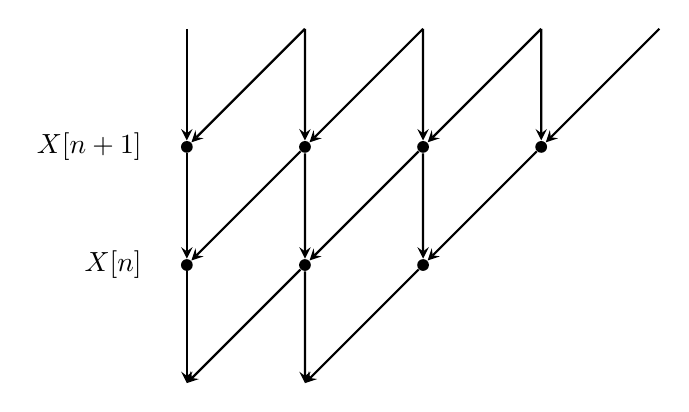
\begin{tikzpicture}[
    scale=1.5,
    dot/.style={circle, fill=black, inner sep=1.5pt},
    arrow/.style={->, thick, >=stealth}
]

% Labels
\node[left] at (-0.3, 1) { $X[n+1]$};
\node[left] at (-0.3, 0) { $X[n]$};

% Nodes for X[n+1]
\node[dot] (n1_1) at (0, 1) {};
\node[dot] (n1_2) at (1, 1) {};
\node[dot] (n1_3) at (2, 1) {};
\node[dot] (n1_4) at (3, 1) {};

% Nodes for X[n]
\node[dot] (n0_1) at (0, 0) {};
\node[dot] (n0_2) at (1, 0) {};
\node[dot] (n0_3) at (2, 0) {};

% Incoming arrows to top row (X[n+1])
\foreach \i in {1,2,3,4} {
    % Vertical arrows from above
    \draw[arrow] (n1_\i |- 0, 2) -- (n1_\i);
    % Diagonal arrows from above-right
    \draw[arrow] ([xshift=1cm, yshift=1cm]n1_\i.center) -- (n1_\i);
}

% Arrows from X[n+1] to X[n]
% Vertical connections
\draw[arrow] (n1_1) -- (n0_1);
\draw[arrow] (n1_2) -- (n0_2);
\draw[arrow] (n1_3) -- (n0_3);

% Diagonal connections
\draw[arrow] (n1_2) -- (n0_1);
\draw[arrow] (n1_3) -- (n0_2);
\draw[arrow] (n1_4) -- (n0_3);

% Outgoing arrows from bottom row (X[n])
% Vertical arrows continuing down
\draw[arrow] (n0_1) -- (0, -1);
\draw[arrow] (n0_2) -- (1, -1);

% Diagonal arrow continuing down-left
\draw[arrow] (n0_3) -- (1, -1);
\draw[arrow] (n0_2) -- (0, -1);

\end{tikzpicture}
\caption{The dots represent $X[n]_j^\circ$. The vertical arrows are $\pi_{n,j,0}$ and the slanted arrows are $\pi_{n,j,1}$.}
\end{figure}
\medskip

Here we say that a morphism $f:U\to Y$ is \emph{motivially locally trivial} if it factors as
$$U\hookrightarrow X \stackrel{g}{\longrightarrow} Y$$
such that $U$ is open in $X$ and that the morphisms $g$ and $g|_{X-U}$ are Zariski locally trivial. 
Then for any motivic invariant $\HH$, we have $\HH_U=\HH_F\cdot\HH_Y$ where $F$ denotes the fiber of $f$ if $Y$ is connected. 

By \eqref{m3}, we have
\beq\label{m4}
\HH_{X[n+1]_j^\circ}=A_{n,j}\HH_{X[n]_j^\circ}+ B_{n,j}\HH_{X[n]_{j-1}^\circ}.\eeq
If $A_{n,j}$ and $B_{n,j}$ are polynomials in $j$, then we will see that \eqref{m4} induces a recursive formula for $\FF_{X[n]}$, which is an effective way of computing $\FF_{X[n]}$ and $\HH_{X[n]}=\FF_{X[n]}(1)$.

\medskip

In the subsequent sections, we will use \eqref{m4} to deduce formulae for stratified motivic invariants of 
the moduli spaces of stable curves of genus $0$ and the Fulton-MacPherson varieties. 


\bigskip

\section{Moduli spaces of stable curves of genus 0}
A fundamental example of an echelon tower is the moduli spaces $\Mbarzn$ of stable curves of genus $0$ with $n$ marked points for $n\ge 3$. Recall that $\Mbarzn$ consists of connected trees of projective lines with $n$ ordered smooth distinct marked points, each of whose irreducible components contains at least three special (nodal or marked) points. It compactifies the moduli space $\cM_{0,n}$ of $n$ distinct ordered points in $\PP^1$ up to projective equivalence. 

To each $C\in \Mbarzn$, we can associate its dual graph whose vertices (resp. edges, ordered legs) correspond to irreducible components (resp. nodes, marked points). For a graph $\gamma$, let $e_\gamma$ denote the number of edges. Since the genus is 0, the dual graph is always a tree and the number of vertices is $e_\gamma+1$. 
For each tree $\gamma$ with $n$ ordered legs, let $\cM_{0,n,\gamma}$ be the locus of $C\in \Mbarzn$ whose dual graph is $\gamma$. Then we have
$$\cM_{0,n,\gamma}=\prod_{v\in \gamma}\cM_{0,k(v)}$$
where $k(v)$ denotes the sum of the number of nodes and the number of marked points in 
the irreducible component corresponding to a vertex $v$.  In particular, $\cM_{0,n,\gamma}$ is a smooth subvariety of codimension $e_\gamma$ in $\Mbarzn$.
Let 
\beq\label{m6}
\cM_{0,n,j}=\bigsqcup_{\gamma:e_\gamma=j}\cM_{0,n,\gamma}.\eeq
Then we have a stratification 
\beq\label{m9}
\Mbarzn=\bcM_{0,n,0}\supset \bcM_{0,n,1}\supset \bcM_{0,n,2}\supset\cdots\supset \bcM_{0,n,n-3}\supset \bcM_{0,n,n-2}=\emptyset\eeq
with $\cM_{0,n}=\cM_{0,n,0}$ and the stratified motivic invariant of $\Mbarzn$ is defined as
\beq\label{m8}
\FF_{\Mbarzn}(y) =\sum_{j=0}^{n-3} y^j\HH_{\cM_{0,n,j}}. 
\eeq

For $n\ge 3$, we have the morphism $$\pi_n:\bcM_{0,n+1}\lra \Mbarzn$$ which forgets the last marked point. 
For $C\in \bcM_{0,n+1}$, $\pi_n(C)$ is obtained by contracting the component in $C$ containing the last marked point if it has only three special points. Otherwise, the underlying curves of $C$ and $\pi_n(C)$ are the same. 
Thus we find that 
$$\cM_{0,n+1,j} =  \left(\cM_{0,n+1,j}\cap \pi_n^{-1}(\cM_{0,n,j})\right) \cup \left(\cM_{0,n+1,j}\cap \pi_n^{-1}(\cM_{0,n,j-1})\right)$$
and obtain morphisms
\beq\label{m5} \pi_{n,j,0}: \cM_{0,n+1,j}\cap \pi_n^{-1}(\cM_{0,n,j})\lra \cM_{0,n,j},\eeq
\[ \pi_{n,j,1}: \cM_{0,n+1,j}\cap \pi_n^{-1}(\cM_{0,n,j-1})\lra \cM_{0,n,j-1}.\]

By fixing the first three marked points at $0,1,\infty$, the open moduli space $\cM_{0,n}$ can be identified with 
$$(\CC-\{0,1\})^{n-3}-\bigcup_{i<j}\{(p_4,\cdots,p_n)\,|\,p_i=p_j\}$$
and $\pi_n:\cM_{0,n+1}\to \cM_{0,n}$ is the restriction of the projection $\cM_{0,n}\times (\CC-\{0,1\})\to \cM_{0,n}$ to the complement of $n-3$ sections.  
Hence, $\pi_n:\cM_{0,n+1}\to \cM_{0,n}$ is motivically locally trivial and 
$$\HH_{\cM_{0,n+1}}=\HH_{\cM_{0,n}} (\LL-n+1),\quad \LL=\HH_\CC.$$
By induction with $\cM_{0,3}=\mathrm{pt}$, we find that 
$$\HH_{\cM_{0,n+1}}=\prod_{j=2}^{n-1}(\LL -j)=\frac{n!}{\LL(\LL-1)}\binom{\LL}{n}.$$
Likewise, by \eqref{m6}, we can decompose \eqref{m5} into the unions of morphisms over $\cM_{0,n,\gamma}$ for $e_\gamma=j$ or $j-1$ and find that the morphisms in \eqref{m5} are motivically locally trivial. The fiber over $C\in \cM_{0,n,j}$ of $\pi_{n,j,0}$ is $C$ minus the $n+j$ special points and has the motivic invariant $$(j+1)\LL -j -n+1.$$ 
The fiber over $C\in \cM_{0,n,j-1}$ of $\pi_{n,j,1}$ consists of $n+j-1$ special points. 
So we proved the following.
\begin{proposition}\label{m15} The moduli spaces $\bcM_{0,n}$ for $n\ge 3$ form a solid echelon tower of stratified varieties and the motivic invariants of strata satisfy  
\beq\label{m7}
\HH_{\cM_{0,n+1,j}}=\left((j+1)\LL -j -n+1\right) \HH_{\cM_{0,n,j}} + (n+j-1)\HH_{\cM_{0,n,j-1}}.
\eeq
\end{proposition}

By \eqref{m7}, we have  
$$\FF_{\bcM_{0,n+1}}=\sum_j y^{j}\HH_{\cM_{0,n+1,j}}=\sum_j(j(\LL-1)+\LL -n+1)y^{j}\HH_{\cM_{0,n,j}}
+\sum_j (n+j-1)y^j\HH_{\cM_{0,n,j-1}}$$
$$=(\LL-1)y\sum_jjy^{j-1}\HH_{\cM_{0,n,j}}+(\LL -n+1)\sum_jy^j\HH_{\cM_{0,n,j}}$$ 
$$+ny\sum_jy^{j-1}\HH_{\cM_{0,n,j-1}}+y^2\sum_j (j-1)y^{j-2}\HH_{\cM_{0,n,j-1}}$$
\[
=(ny-n+1+\LL)\FF_{\Mbarzn}+y(y+\LL-1)\,\partial_y\FF_{\Mbarzn}.\]
So we obtain the following.
\begin{theorem}\label{m14}
    The stratified motivic invariants $\FF_{\Mbarzn}(y)$ of $\Mbarzn$ are uniquely determined by the inductive formula
    \beq\label{m11} \FF_{\bcM_{0,n+1}} = (ny-n+1+\LL)\FF_{\Mbarzn}+y(y+\LL-1)\,\partial_y\FF_{\Mbarzn}, \quad \FF_{\bcM_{0,3}}=1.\eeq
\end{theorem}
For example, $\FF_{\bcM_{0,4}}=(\LL-2)+3y$ and 
$$\FF_{\bcM_{0,5}}=(\LL-2)(\LL-3)+(10\LL-20)y+15y^2.$$

Note that the right hand side of \eqref{m11} equals $$((n-1)y-n+2)\FF_{\Mbarzn}+(y+\LL-1)\partial_y(y\FF_{\Mbarzn})$$
since $\partial_y(y \FF_{\Mbarzn})=\FF_{\Mbarzn}+y\partial_y\FF_{\Mbarzn}$. Multiplying $y$, we obtain 
$$y\FF_{\bcM_{0,n+1}}=((n-1)y-n+2)y\FF_{\Mbarzn}+y(y+\LL-1)\partial_y(y\FF_{\Mbarzn}).$$
Let $F_{n}(y)=y\FF_{\bcM_{0,n+1}}(y)$. Then we have 
\beq\label{m10}
F_{n+1}(y)=(ny-n+1)F_n(y)+y(y+\LL-1)\partial_yF_n(y), \quad F_2(y)=y\FF_{\bcM_{0,3}}=y. 
\eeq
Note that \eqref{m10} is precisely the defining inductive formula for the bivariate deformation $F_n(y,t)$ of the even degree Poincar\'e polynomial of $\bcM_{0,n+1}$ in \cite[Definition 2.2]{BercziKiem2026} when $\HH$ is the virtual Poincar\'e polynomial. So we proved the following.
\begin{corollary}\label{m17}
    The bivariate deformation $F_n(y,t)$ of the even degree Poincar\'e polynomial %\eqref{i7} $\sum_{i}t^i\dim H^{2i}(\bcM_{0,n+1})$ 
    of $\bcM_{0,n+1}$ in \cite{BercziKiem2026} is uniquely determined by   $F_n(y,t^2)=y\FF_{\bcM_{0,n+1}}(y)$ when $\HH$ is the virtual Poincar\'e polynomial.   
\end{corollary}
Consequently, the coefficient of $y^{j+1}$ in $F_n(y,t)$ is the virtual Poincar\'e polynomial of $\cM_{0,n+1,j}$:
\beq\label{m12}
[y^{j+1}]F_n(y,t^2)=P_{\cM_{0,n+1},j}({t}).\eeq
Thus Corollary \ref{m17} provides us with a geometric meaning of the coefficients of $F_n(y,t)$. 

See \cite{BercziKiem2026} 
for the generating function $$\Phi(x,y)=x+\sum_{n\ge 2}\frac{x^n}{n!}y\FF_{\bcM_{0,n+1}}(y),$$ the partial differential equation satisfied by $\Phi$, and a proof of the real-rootedness of the Poincar\'e polynomial of $\Mbarzn$ as an application.
We can recover all the previously known formulae for the Poincar\'e polynomial of $\Mbarzn$ from \eqref{m7} or \eqref{m11} by using the computation in \cite{BercziKiem2026}. 

\begin{remark}\label{m18}
    The moduli spaces $\Mbargn$ also form an echelon tower which is not solid. Everything holds except that the morphism $$\pi_{n,j,0}:\cM_{g,n+1,j}\cap \pi_n^{-1}(\cM_{g,n,j})\lra \cM_{g,n,j}$$
    is not motivically locally trivial where $\pi_n:\bcM_{g,n+1}\to \Mbargn$ denotes the forgetful morphism. Likewise, the moduli spaces of stable maps $\bcM_{g,n}(Y,d)$ for a convex smooth projective variety $Y$ form an echelon tower that is not solid. 
\end{remark}

\bigskip


\section{Stratified motivic invariants of Fulton-MacPherson varieties}

In this section, we fix a motivic invariant $\HH$ and determine the stratified motivic invariants of the Fulton-MacPherson varieties. 

For a smooth projective variety $Y$ of dimension $m$, let $Y[n]$ denote the Fulton-MacPherson compactification of the configuration space 
$$Y[n]^\circ=Y^n-\bigcup_{i<j}\Delta_{ij},\quad \Delta_{ij}=\{(p_1,\cdots,p_n)\,|\,p_i=p_j\}$$
of $n$ ordered distinct points in $Y$ (cf. \cite{FultonMacpherson1994}). 
Each element in $Y[n]$ parameterizes a variety $Y'$, obtained from $Y$ by repeatedly blowing up at a smooth point and gluing $\PP^m$ along the exceptional divisor, together with $n$ smooth distinct marked points $p_i$ such that the automorphism group is trivial. 

\begin{center}
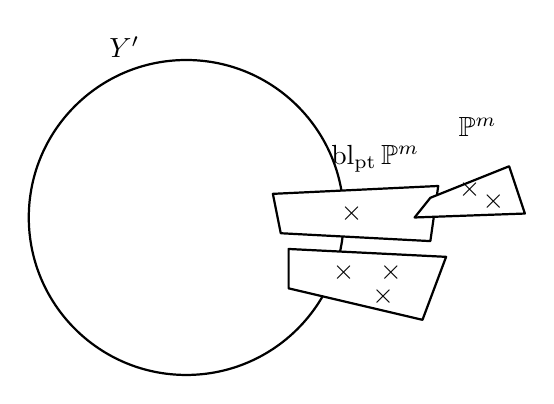
\begin{tikzpicture}[line cap=round, line join=round, >=stealth]

  % 1. Draw the main variety Y' (large circle)
  \draw[thick] (0,0) circle (2cm);
  \node at (110:2.3) {$Y'$};

  % 2. Draw the vertical connecting line between the two main wedges
  % (This is drawn first so the white-filled wedges clean up the ends)
%  \draw[thick] (1.8, -0.2) -- (1.8, -0.5);

  % 3. Lower Wedge
  \filldraw[fill=white, thick] (1.3, -0.4) -- (3.3, -0.5) -- (3.0, -1.3) -- (1.3, -0.9) -- cycle;
  
  % Marks in Lower Wedge
  \node at (2.0, -0.7) {$\times$};
  \node at (2.6, -0.7) {$\times$};
  \node at (2.5, -1.0) {$\times$};

  % 4. Middle Wedge (bl_pt P^n)
  \filldraw[fill=white, thick] (1.1, 0.3) -- (3.2, 0.4) -- (3.1, -0.3) -- (1.2, -0.2) -- cycle;
  \node[anchor=south] at (2.4, 0.45) {$\operatorname{bl}_{\operatorname{pt}} \mathbb{P}^m$};
  
  % Mark in Middle Wedge
  \node at (2.1, 0.05) {$\times$};

  % 5. Top-Right Wedge (P^n) - Overlaps the Middle Wedge
  \filldraw[fill=white, thick] (2.9, 0.0) -- (3.1, 0.25) -- (4.1, 0.65) -- (4.3, 0.05) -- cycle;
  \node[anchor=south] at (3.7, 0.9) {$\mathbb{P}^m$};

  % Marks in Top-Right Wedge
  \node at (3.6, 0.35) {$\times$};
  \node at (3.9, 0.2) {$\times$};

\end{tikzpicture}
\end{center}

For $(Y',p_1,\cdots, p_n)\in Y[n]$, let $\gamma_{Y'}$ be its dual graph whose vertices (resp. edges, legs) correspond to the irreducible components (resp. intersections $\PP^{m-1}$ of irreducible components, marked points) in $Y'$. There is a distinguished vertex representing (a blowup of) $Y$, called the distinguished component. The graph $\gamma_{Y'}$ is always a tree. 

%Let $X=Y[n]$. 
For a tree $\gamma$ with $n$ legs and a distinguished vertex, let $Y[n]^\circ_\gamma$ be the subset of $Y[n]$ consisting of objects whose dual graph is $\gamma$.  
Then $Y[n]$ is stratified by  %closed subvarieties   
$$Y[n]_j=\bigsqcup_{\gamma: e_\gamma\ge j} Y[n]^\circ_\gamma, \quad Y[n]^\circ_j=\bigsqcup_{\gamma: e_\gamma= j} Y[n]^\circ_\gamma$$
where $e_\gamma$ is the number of edges in $\gamma$.

Let $\pi_n:Y[n+1]\to Y[n]$ denote the morphism forgetting the last marked point $p_{n+1}$. If the irreducible component containing $p_{n+1}$ stays stable (i.e. the autormorphism group is trivial) after deleting it, the underlying variety remains the same. If not, we contract the irreducible component. Therefore, we have   
$$\pi_n\left( Y[n+1]^\circ_j\right) \subset Y[n]^\circ_j\sqcup Y[n]^\circ_{j-1}$$
so that 
\beq\label{f2}
Y[n+1]_j^\circ=\left(Y[n+1]_j^\circ\cap \pi_n^{-1}(Y[n]^\circ_j) \right)\sqcup \left(Y[n+1]_j^\circ\cap \pi_n^{-1}(Y[n]^\circ_{j-1}) \right).
\eeq 
Then $\pi_n$ induces morphisms 
\beq\label{f16}
\pi_{n,j,0}:Y[n+1]_j^\circ\cap \pi_n^{-1}(Y[n]^\circ_j) \lra Y[n]^\circ_j, 
\quad \pi_{n,j,1}:Y[n+1]_j^\circ\cap \pi_n^{-1}(Y[n]^\circ_{j-1}) \lra Y[n]^\circ_{j-1}\eeq 
As in the previous section, we can further decompose these into morphisms over $Y[n]^\circ_\gamma$ where $\gamma$ runs over trees with $e_\gamma=j, j-1$.  
The fiber of $\pi_{n,j,0}$ over $(Y',p_1,\cdots,p_n)$ is the complement in $Y'$ of  the marked points and the intersections of irreducible components in $Y'$. It is the same as the disjoint union of $Y$ and $j$ copies of $\PP^{m}$ minus $j$ points (blowup centers), $j$ copies of $\PP^{m-1}$ (intersections of irreducible components) and $n$ marked points. 
We thus find that $\pi_{n,j,0}$ is motivically locally trivial whose fibers have the motivic invariant
\beq\label{f4}
\HH_Y-j+j\HH_{\CC^m}-n=\HH_Y-n+j(\LL^m-1).
\eeq
The fiber of $\pi_{n,j,1}$ over $(Y',p_1,\cdots,p_n)$ consists of $(\widetilde{Y}',p_1,\cdots,p_{n+1} )\in Y[n+1]_j^\circ$ 
where $\widetilde{Y}'\to Y'$ contracts the irreducible component containing $p_{n+1}$ which has exactly one more marked point or one irreducible component connected in the direction away from the distinguished component.  
The contracted component is mapped to a marked point by the contraction $\widetilde{Y}'\to Y'$ in the former case and to the intersecting $\PP^{m-1}$ in the latter case. The automorphism group of $\PP^{m}$ fixing $\PP^{m-1}\cup\mathrm{pt}$ pointwisely or that of $\mathrm{bl}_{\mathrm{pt}}\PP^m$ fixing $\PP^{m-1}\cup E$ pointwisely is $\CC^*$ where $E$ denotes the exceptional divisor and so we find that 
$\pi_{n,j,1}^{-1}(Y',p_1,\cdots,p_n)$ is the union of 
of $n+j-1$ copies of $\PP^{m-1}=(\PP^m-\PP^{m-1}\cup \mathrm{pt})/\CC^*=(\mathrm{bl}_{\mathrm{pt}}\PP^m-\PP^{m-1}\cup E)/\CC^*$, each corresponding to a leg or an edge of the dual graph of $(Y',p_1,\cdots,p_n)$. 
We thus find that $\pi_{n,j,1}$ is also motivically locally trivial and 
the fibers have the motivic invariant 
\beq\label{f4'}
(n+j-1)\,\HH_{\PP^{m-1}}.
\eeq
Therefore we have
\beq\label{f5}
\HH_{Y[n+1]_j^\circ}= \left( \HH_Y-n+j(\LL^m-1) \right) \HH_{Y[n]^\circ_j} +
(n+j-1) \HH_{\PP^{m-1}} \HH_{Y[n]^\circ_{j-1}} 
\eeq
which immediately implies 
%$$\FF_{Y[n+1]}(y,u,v)=\sum_j \left( \HH_Y-j+j(uv)^d-n \right) y^j\HH_{Y[n]^\circ_j} +
%\sum_j(j-1+n)y^j \HH_{\PP^{d-1}} \HH_{Y[n]^\circ_{j-1}}.$$
%Therefore we proved 
the following inductive formula for the Fulton-MacPherson space $Y[n]$ by a computation similar to that for \eqref{m10}.
\begin{theorem}\label{f8} The Fulton-MacPherson varieties $Y[n]$ form a solid echelon tower of stratified varieties.  
The stratified motivic invariant 
$\FF_{Y[n]}=\sum_j y^j\HH_{Y[n]_j^\circ}$ of $Y[n]$  is uniquely determined by the recursive formula
\beq\label{f6} 
\FF_{Y[n+1]}=\left(\HH_Y-n+ny\HH_{\PP^{m-1}}\right)\FF_{Y[n]}+ y\left(y\HH_{\PP^{m-1}}+ ({\LL^m}-1)\right)\partial_y\FF_{Y[n]}\eeq
with $\FF_{Y[1]}=\HH_Y$. 
\end{theorem}
Since $\FF_{Y[n]}(1)$ is the Hodge polynomial of ${Y[n]}$ when $\HH$ is the Hodge-Deligne polynomial, \eqref{f6} gives us an effective way of computing the Hodge and Poincar\'e polynomials of the Fulton-MacPherson variety $Y[n]$.

For example, when $Y=\PP^1$, \eqref{f6} is 
\beq\label{f17}
\FF_{\PP^1[n+1]}=(\LL+1-n+ny)\FF_{\PP^1[n]} + y(y+\LL-1)\partial_y\FF_{\PP^1[n]}.\eeq
%recovers \eqref{eq:FM-residual-recurrence-section} with $\widehat{F}$ replaced by $\FF$.


\medskip

\noindent\textbf{Example.}
Since $Y[1]=Y$ is smooth, $\FF_{Y}=\HH_Y$. 
For $n=1$, \eqref{f6} is 
$$\FF_{Y[2]}=(\HH_Y-1+y\HH_{\PP^{m-1}})\HH_Y$$ which also follows from the blowup construction $Y[2]=\mathrm{bl}_Y(Y\times Y)$. 

For $n=2$, \eqref{f6} gives
$$\FF_{Y[3]}=(\HH_Y-2+2y\HH_{\PP^{m-1}})(\HH_Y-1+y\HH_{\PP^{m-1}})\HH_Y + \left(y^2\HH_{\PP^{m-1}}+ y(\LL^m-1)\right)\HH_{\PP^{m-1}}\HH_Y$$
$$=\HH_Y(\HH_Y-1)(\HH_Y-2)
+y(\LL^m+3\HH_Y-5)\HH_{\PP^{d-1}}\HH_Y
+3y^2\HH_{\PP^{d-1}}^2\HH_Y.$$
Letting $y=1$, we find that the Hodge polynomial of $Y[3]$ equals
$$\HH_Y^3+\HH_Y(\HH_{\PP^{2m-1}}-1)+3(\HH_Y^2+\HH_Y(\HH_{\PP^{m-1}}-1))(\HH_{\PP^{m-1}}-1)$$
which can be also read off from the blowup construction of $Y[3]$. In fact, $Y[3]\to Y^3$ is the composition of two blowups, first along the small diagonal $\Delta_{123}\cong Y$ and then along the union of the proper transforms of $\Delta_{12}$, $\Delta_{23}$ and $\Delta_{13}\cong Y^2$. 

\medskip

It is useful to define the generating function of all $\FF_{Y[n]}$. 
\begin{definition}
\beq\label{f18} \Psi(x,y)=1+\sum_{n\ge 1}\frac{x^n}{n!}\FF_{Y[n]}(y)\  \in \ R[y][\![x]\!].\eeq
\end{definition}
Then it is easy to check that \eqref{f6} is equivalent to the following partial differential equation.
\begin{proposition}
\beq\label{f7}
\HH_Y\Psi=(1+x(1-y\HH_{\PP^{m-1}}))\partial_x\Psi - y(y\HH_{\PP^{m-1}}+{\LL^m}-1)\partial_y\Psi.
\eeq
Moreover, $\Psi$ is uniquely determined by \eqref{f7} and $\Psi|_{x=0}=1$. 
\end{proposition}

When $Y=\PP^1$, \eqref{f7} gives 
$$(\LL+1)\Psi=(1-(y-1)x)\partial_x\Psi-y(y+\LL-1)\partial_y\Psi$$
and hence we find that \eqref{f18} coincides with the generating function $\Psi$ in \cite[\S5]{BercziKiem2026} with $t$ replaced by $\LL$. % when $\HH$ is the virtual Poincar\'e polynomial.
Since the coefficient of $\frac{x^n}{n!}$ in $\Psi$ is the bivariate deformation of the Poincar\'e polynomial of $\PP^1[n]$, we obtain the following.
\begin{corollary}\label{f21}
  The bivariate deformation $\widetilde{F}_n(y,t^2)$ of the Poincar\'e polynomial of $\PP^1[n]$ in \cite{BercziKiem2026} is precisely the stratified virtual Poincar\'e polynomial $\FF_{\PP^1[n]}(y,t)$.   
\end{corollary}

We end this paper with a new proof of Manin's formulae for the Poincar\'e polynomial of the Fulton-MacPherson variety $Y[n]$ in \cite{Manin1999}, from \eqref{f7}.

It is useful to define $\Phi\in R[y][\![x]\!]$ as the unique series satisfying
$$\Psi=(1+\Phi)^{\HH_Y}$$
when $\HH_Y\ne 0$.  
Then \eqref{f7} is equivalent to 
\beq\label{f9}
1+\Phi = (1+x(1-y\HH_{\PP^{m-1}}))\partial_x\Phi - y(y\HH_{\PP^{m-1}}+{\LL^m}-1)\partial_y\Phi.
\eeq

As in \cite{BercziKiem2026}, we can solve this partial differential equation along $y=1$ by using the characteristic equations: 
\beq\label{f11} \frac{dx}{ds}=1+x(1-y\HH_{\PP^{m-1}}),\quad \frac{dy}{ds}=- y(y\HH_{\PP^{m-1}}+{\LL^m}-1),\quad \frac{d\Phi}{ds}=1+\Phi.\eeq
Let $x=0$ at $s=0$ so that $\Phi=0$ at $s=0$ as well. Then the last equation gives us 
\beq\label{f10}
\Phi=e^s-1=u-1.\eeq
We can also solve the second equation in \eqref{f11} as
\beq\label{f12}
\frac{y}{y+\LL-1} = \frac{1}{\LL} \left( \frac{z}{u} \right)^{\LL^m-1}\eeq
where $z$ is the value of $u=e^s$ when $y(s)=1$, i.e. $y(\log z)=1$. 

From the first equation in \eqref{f11}, we have
\beq\label{f13}
\frac{dx}{du} + \frac{y\HH_{\PP^{m-1}} -1 }{u} x =\frac{1}{u}\eeq 
From \eqref{f12}, we find that 
$$y\HH_{\PP^{m-1}} -1  = \frac{\LL^m\left( \frac{z}{u} \right)^{\LL^m-1}-\LL}{\LL-\left( \frac{z}{u}\right) ^{\LL^m-1}}.$$
We thus have 
\beq\label{f14} \exp \int \frac{y\HH_{\PP^{m-1}} -1}{u}  \,du = \frac{z}{u}\left( \LL - \left(\frac{z}{u}\right)^{\LL^m-1}\right).\eeq
By multiplying \eqref{f14} to \eqref{f13} and integrating from $u=1$ to $u=z$ while remembering $x=0$ when $u=1$, we obtain
$$(\LL-1)x=\int_{u=1}^{u=z} \frac{z}{u^2}\left( \LL - \left(\frac{z}{u}\right)^{\LL^m-1}\right) \,du =\frac{\LL^{m+1}(z-1)-z^{\LL^m}+1}{\LL^m}.$$
We thus find that $\phi:=\Phi|_{y=1}=z-1$ satisfies  
\beq\label{f15}
x=\frac{\LL^{m+1}\phi-(1+\phi)^{\LL^m}+1}{\LL^m(\LL-1)}, \quad \psi:=\Psi|_{y=1}=(1+\phi)^{\HH_Y}.
\eeq 
When $\HH$ is the Hodge-Deligne polynomial, we have 
\beq\label{f20} \psi(x)=1+\sum_{n\ge 1}\frac{x^n}{n!}\HH_{Y[n]}.\eeq 
%Thus \eqref{f15} recovers Manin's formulae for the Poincar\'e polynomial of the Fulton-MacPherson space $Y[n]$.
Therefore, we proved the following.
\begin{theorem} \cite[(4.22) and (4.24)]{Manin1999}
    The Hodge polynomials and the Poincar\'e polynomials $\HH_{Y[n]}$ of $Y[n]$ are uniquely determined by \eqref{f15} and \eqref{f20}.
\end{theorem}


\bigskip







\bibliographystyle{amsalpha}
\bibliography{references}





\end{document}










\bibliographystyle{amsplain}
\begin{thebibliography}{99}
\bibitem{BercziKiem2026} G. B\'erczi and Y.-H. Kiem, {\em Real-rootedness of the Poincar\'e polynomials of $\overline{\mathcal M}_{0,n}$: an AI-assisted proof}, preprint, arXiv: 2605.29151.
\bibitem{FultonMacpherson1994} W. Fulton and R. MacPherson, {\em A compactification of configuration spaces}, Annals of Mathematics, Second Series (1994), 183--225. 
\bibitem{Manin1999} Y. Manin. {\em Frobenius Manifolds, Quantum Cohomology, and Moduli Spaces}. AMS Colloquium Publ. 47, Providence, RI.
\end{thebibliography}









\section{Stratified motivic invariants of moduli spaces of stable maps}


Let $Y$ be a convex variety, i.e. for any morphism $f:\PP^1\to Y$, $H^1(f^*T_Y)=0$. 
Let $\Mbarzn(Y,d)$ be the moduli space of stable maps $f:C\to Y$ of genus 0 with $n$ marked points and $f_*[C]=d\in H_2(Y,\ZZ)$. Then $X[n]=\Mbarzn(Y,d)$ admits a stratification where $X[n]_j^\circ$ consists of stable maps $f:C\to Y$ from prestable curves $C$ with $j$ nodes. 


Consider the morphism $$\pi_n:\bcM_{0,n+1}(Y,d)\lra \Mbarzn(Y,d)$$
which forgets the last marked point. 
Let $f\in \bcM_{0,n+1}(Y,d)$. 
If the last marked point is contained in an irreducible component with exactly three special points (i.e. nodes or marked points) which is contracted by $f$, then $\pi_n(f)\in \Mbarzn(Y,d)_{j-1}^\circ$. Otherwise, $\pi_n(f)\in \Mbarzn(Y,d)_j^\circ$. 







\section{Fulton--MacPherson spaces and the residual deformation}

Let
\[
  X_n=\PP^1[n]\cong \bcM_{0,n}(\PP^1,1)
\]
be the Fulton--MacPherson compactification of the configuration space of
$n$ ordered points in $\PP^1$, equivalently the moduli space of genus-zero
$n$-pointed stable maps to $\PP^1$ of degree $1$.  For
\[
  f:(C,p_1,\ldots,p_n)\longrightarrow \PP^1
\]
in $X_n$, there is a unique irreducible component $C_0\subset C$ on which
$f$ has degree $1$; this component maps isomorphically to $\PP^1$.  All
other irreducible components are contracted.  We write
\[
  c(f)=\#\{\text{contracted irreducible components of } C\}.
\]
For $0\le q\le n-1$, let
\[
  X_{n,q}=\{f\in X_n\mid c(f)=q\}.
\]
This is a union of locally closed stable-map strata.  We also fix the first
evaluation map
\[
  \mathrm{ev}_1:X_n\longrightarrow \PP^1,
  \qquad
  \mathrm{ev}_1(f)=f(p_1),
\]
and put
\[
  X_{n,q}^{\infty}=X_{n,q}\cap \mathrm{ev}_1^{-1}(\infty).
\]

Let
\[
  \Phi(x,y,t)=\sum_{m\ge 1}F_m(y,t)\frac{x^m}{m!},
\]
where the polynomials $F_m(y,t)$ are the bivariate deformations in Theorem \ref{10}, with the convention
$F_1(y,t)=1$.  Define the Fulton--MacPherson deformation $\Ft_n(y,t)$ by
\begin{equation}\label{eq:FM-Psi-def}
  (1+\Phi(x,y,t))^{t+1}
  =1+\sum_{n\ge 1}\Ft_n(y,t)\frac{x^n}{n!}.
\end{equation}
By definition, after setting $y=1$, one obtains the Poincar\'e polynomial of
$X_n$:
\[
  \Ft_n(1,u^2)=\PP_u(X_n).
\]
We write
\[
  \Pt_n(t):=\Ft_n(1,t).
\]
The polynomials $\Ft_n(y,t)$ are all divisible by $t+1$.  Indeed,
\[
  (1+\Phi)^{t+1}-1
  =\sum_{k\ge 1}\binom{t+1}{k}\Phi^k,
  \qquad
  \binom{t+1}{k}=\frac{(t+1)t(t-1)\cdots(t-k+2)}{k!}.
\]
We therefore define the residual Fulton--MacPherson deformation by
\begin{equation}\label{eq:FM-residual-def}
  \widehat\Psi(x,y,t)
  :=\frac{(1+\Phi(x,y,t))^{t+1}-1}{t+1}
  =\sum_{n\ge 1}\widehat F_n(y,t)\frac{x^n}{n!},
\end{equation}
so that $\widehat F_n(y,t)=\Ft_n(y,t)/(t+1)$.  On the slice $y=1$ we write
\[
  \widehat P_n(t):=\widehat F_n(1,t)=\frac{\Pt_n(t)}{t+1}.
\]

\begin{theorem}[Coefficient interpretation for the FM deformation]
\label{prop:FM-coefficient-interpretation}
For every $n\ge 1$ and every $0\le q\le n-1$, we have
\begin{equation}\label{eq:FM-coeff-full}
  [y^q]\Ft_n(y,u^2)=\PP_u(X_{n,q})
\end{equation}
and
\begin{equation}\label{eq:FM-coeff-residual}
  [y^q]\widehat F_n(y,u^2)=\PP_u(X_{n,q}^{\infty}).
\end{equation}
In particular,
\[
  \widehat F_n(1,u^2)=\PP_u\bigl(\mathrm{ev}_1^{-1}(\infty)\bigr).
\]
Thus the residual deformation has the following modular meaning: the
coefficient of $y^q$ is the virtual Poincar\'e polynomial of the locus of
stable maps whose source curve has precisely $q$ contracted components, after
fixing the image of the first marking to be $\infty$.
\end{theorem}

\begin{proof}
Let $\Pi_n$ be the set of set partitions of $\{1,\ldots,n\}$.  Given
$f\in X_n$, two markings $p_i,p_j$ determine the same block precisely when
their images on the degree-one component coincide.  Thus a partition
\[
  \pi=\{B_1,\ldots,B_k\}\in \Pi_n
\]
records the $k$ support points on the component $C_0\cong \PP^1$.
For a block $B$ of size $m$, the contracted tree attached over the
corresponding support point is a rooted stable rational curve with $m$ labelled
markings and one additional root marking, hence is parametrized by
$\Mbar_{0,m+1}$.  When $m=1$ there is no contracted component over that
support point, and this agrees with the convention $F_1(y,t)=1$.
For $m\ge 2$, the interpretation \eqref{10} says that the coefficient of
$y^v$ in $F_m(y,u^2)$ is the virtual Poincar\'e polynomial of the locus of
rooted bubble trees with exactly $v$ irreducible components.  These components
are precisely the contracted components of the stable map.

For a fixed partition $\pi$ with $k$ blocks, the support points form the
ordered configuration space of $k$ distinct points of $\PP^1$, ordered by the
blocks of $\pi$.  Its virtual Poincar\'e polynomial is
\[
  \PP_u(\operatorname{Conf}_k(\PP^1))
  =(t+1)t(t-1)\cdots(t-k+2),
  \qquad t=u^2.
\]
Therefore the contribution of all stable maps with support partition $\pi$ is
\[
  (t+1)t(t-1)\cdots(t-k+2)\prod_{B\in \pi}F_{|B|}(y,t).
\]
Summing over all partitions gives
\begin{equation}\label{eq:FM-partition-full}
  \sum_{q\ge 0}y^q\PP_u(X_{n,q})
  =
  \sum_{\pi\in\Pi_n}
  (t+1)t(t-1)\cdots(t-|\pi|+2)
  \prod_{B\in\pi}F_{|B|}(y,t).
\end{equation}
By the exponential formula, the right hand side is exactly the coefficient of
$x^n/n!$ in $(1+\Phi(x,y,t))^{t+1}$.  This proves
\eqref{eq:FM-coeff-full}.

For the residual statement, fix $\mathrm{ev}_1=\infty$.  If $B_0$ is the
block of $\pi$ containing the label $1$, then the support point corresponding
to $B_0$ is forced to be $\infty$.  The remaining $k-1$ support points form
the ordered configuration space of $k-1$ distinct points of
$\mathbb A^1=\PP^1\setminus\{\infty\}$.  Hence
\[
  \PP_u(\operatorname{Conf}_{k-1}(\mathbb A^1))
  =t(t-1)\cdots(t-k+2),
\]
with the convention that this product is $1$ when $k=1$.  Thus
\begin{equation}\label{eq:FM-partition-residual}
  \sum_{q\ge 0}y^q\PP_u(X_{n,q}^{\infty})
  =
  \sum_{\pi\in\Pi_n}
  t(t-1)\cdots(t-|\pi|+2)
  \prod_{B\in\pi}F_{|B|}(y,t).
\end{equation}
Again by the exponential formula, the right hand side is the coefficient of
$x^n/n!$ in
\[
  \frac{(1+\Phi(x,y,t))^{t+1}-1}{t+1}.
\]
This proves \eqref{eq:FM-coeff-residual}.
\end{proof}

\begin{corollary}[Residual recurrence]\label{cor:FM-residual-recurrence}
The residual polynomials satisfy
\begin{equation}\label{eq:FM-residual-recurrence-section}
  \widehat F_{n+1}(y,t)
  =
  (ny-n+t+1)\widehat F_n(y,t)
  +y(y+t-1)\partial_y\widehat F_n(y,t),
  \qquad
  \widehat F_1(y,t)=1.
\end{equation}
\end{corollary}

\begin{proof}
Coefficient extraction from \eqref{8} gives
\[
  \bigl(1-(y-1)x\bigr)\partial_x\Phi
  -y(y+t-1)\partial_y\Phi
  =1+\Phi.
\]
Applying the same differential operator to
$\Psi=(1+\Phi)^{t+1}$ gives
\[
  \bigl(1-(y-1)x\bigr)\partial_x\Psi
  -y(y+t-1)\partial_y\Psi
  =(t+1)\Psi.
\]
Since $\Psi=1+(t+1)\widehat\Psi$, this is equivalent to
\[
  \bigl(1-(y-1)x\bigr)\partial_x\widehat\Psi
  -y(y+t-1)\partial_y\widehat\Psi
  =1+(t+1)\widehat\Psi.
\]
Taking the coefficient of $x^n/n!$ gives \eqref{eq:FM-residual-recurrence-section}.
\end{proof}

\begin{remark}[Small cases]
The first residual polynomials are
\[
  \widehat F_1(y,t)=1,
  \qquad
  \widehat F_2(y,t)=t+y,
\]
\[
  \widehat F_3(y,t)=t(t-1)+(4t-2)y+3y^2.
\]
For $n=2$, the term $t$ is the open stratum where the second support point
moves in $\mathbb A^1$, and the term $y$ is the boundary stratum with one
contracted component over $\infty$.  For $n=3$, the term $t(t-1)$ is
$\operatorname{Conf}_2(\mathbb A^1)$; the coefficient $4t-2$ records the
strata with one contracted component; and the term $3y^2$ is the three-point
boundary of $\Mbar_{0,4}$ over $\infty$.
\end{remark}






\section{Refined Hodge-Deligne polynomials of the Fulton-MacPherson spaces}

Let $X$ be a variety of dimension $N$ over $\CC$. 
A \emph{stratification} of $X$ is a filtration
\beq\label{f1}
X_\cdot: X=X_0\supset X_1\supset X_2\supset \cdots \supset X_N\supset X_{N+1}=\emptyset
\eeq
by closed subvarieties such that $X_j^\circ=X_j-X_{j+1}$ is a smooth quasi-projective variety of dimension $N-j$. Let $X^\circ=X_0^\circ=X-X_1$.
\begin{definition}
Let $(X,X_\cdot)$ be a stratified quasi-projective variety. The \emph{refined Hodge-Deligne polynomial} of $(X,X_\cdot)$ is defined by
$$\FF_X(y,u,v)=\sum_{j=0}^Ny^j\HH_{X_j^\circ}(u,v)=\HH_{X^\circ}(u,v)+y\,\HH_{X_1^\circ}(u,v)+\cdots +y^{N-1}\HH_{X_{N-1}^\circ}(u,v)+y^N\HH_{X_N}(u,v)$$
where $\HH_Z(u,v)$ denotes the Hodge-Deligne polynomial 
$$\HH_Z(u,v)=\sum_{k,p,q}(-1)^ku^{p}v^q\dim H^{p,q;k}_c(Z),\quad H^{p,q;k}(X)=\mathrm{gr}^p_F\mathrm{gr}^W_{p+q}H^k_c(Z).$$
\end{definition}
Here $\mathrm{gr}^p_F$ and $\mathrm{gr}^W_{p+q}$ denote the graded part by the Hodge and weight filtrations respectively of the mixed Hodge structure on $H^k_c(Z)$. 
By definition, 
\begin{enumerate}
    \item[(i)] $\FF_X(1,u,v)=\HH_X(u,v)$ is the Hodge-Deligne polynomial of $X$ and
    \item[(ii)] $\FF_X(0,u,v)=\HH_{X^\circ}(u,v)$ is the Hodge-Deligne polynomial of the interior $X^\circ=X-X_1$.
\end{enumerate}

For a smooth projective variety $Y$ of dimension $d$, let $Y[n]$ denote the Fulton-MacPherson compactification of the configuration space 
$$Y[n]^\circ=Y^n-\bigcup_{i<j}\Delta_{ij},\quad \Delta_{ij}=\{(p_1,\cdots,p_n)\,|\,p_i=p_j\}$$
of $n$ ordered distinct points in $Y$. 
For each $Y'\in Y[n]$, let $\gamma_{Y'}$ be its dual graph whose vertices (resp. edges, legs) correspond to irreducible components (resp. intersections $\PP^{n-1}$ of irreducible components, marked points) of $Y'$. There is a distinguished vertex representing (a blowup of) $Y$ and the graph $\gamma_{Y'}$ is in fact a tree. 

%Let $X=Y[n]$. 
For a tree $\gamma$ with $n$ legs and a distinguished vertex, let $Y[n]_\gamma$ be the subset of $Y[n]$ consisting of objects whose dual graph is $\gamma$.  
Then $Y[n]$ admits a stratification by closed subvarieties   
$$Y[n]_j=\bigsqcup_{\gamma: e_\gamma=j} Y[n]_\gamma$$
where $e_\gamma$ is the number of edges in $\gamma$.

Let $\pi_n:Y[n+1]\to Y[n]$ denote the morphism forgetting the last marked point. Then
$$\pi_n\left( Y[n+1]_j^\circ\right) \subset Y[n]_j^\circ\sqcup Y[n]_{j-1}^\circ$$
so that 
\beq\label{f2}
Y[n+1]_j^\circ=\left(Y[n+1]_j^\circ\cap \pi_n^{-1}(Y[n]^\circ_j) \right)\sqcup \left(Y[n+1]_j^\circ\cap \pi_n^{-1}(Y[n]^\circ_{j-1}) \right).
\eeq 
It is straighforward to see that $\pi_n$ restricts to a motivically Zariski locally trivial fibrations
$$Y[n+1]_j^\circ\cap \pi_n^{-1}(Y[n]^\circ_j) \lra Y[n]^\circ_j, 
\quad Y[n+1]_j^\circ\cap \pi_n^{-1}(Y[n]^\circ_{j-1}) \lra Y[n]^\circ_{j-1}$$
whose fibers respectively have Hodge-Deligne polynomials
\beq\label{f4}
\HH_Y(u,v)-j+j(uv)^d-n \quad \text{and} \quad (j-1+n)\,\HH_{\PP^{d-1}}(u,v).
\eeq
Therefore we have
\beq\label{f5}
\HH_{Y[n+1]_j^\circ}(u,v)= \left( \HH_Y(u,v)-j+j(uv)^d-n \right) \HH_{Y[n]^\circ_j}(u,v) +
(j-1+n) \HH_{\PP^{d-1}}(u,v) \HH_{Y[n]^\circ_{j-1}}(u,v) 
\eeq
which immediately implies 
%$$\FF_{Y[n+1]}(y,u,v)=\sum_j \left( \HH_Y-j+j(uv)^d-n \right) y^j\HH_{Y[n]^\circ_j} +
%\sum_j(j-1+n)y^j \HH_{\PP^{d-1}} \HH_{Y[n]^\circ_{j-1}}.$$
%Therefore we proved 
the following inductive formula for the Fulton-MacPherson space $Y[n]$.
\begin{theorem}\label{f8} 
$\FF_{Y[n]}$ satisfies the recursive formula
\beq\label{f6} 
\FF_{Y[n+1]}=\left(\HH_Y-n+ny\HH_{\PP^{d-1}}\right)\FF_{Y[n]}+ y\left(y\HH_{\PP^{d-1}}+ (\HH_{\CC^d}-1)\right)\partial_y\FF_{Y[n]}\eeq
with $\FF_{Y[1]}=\HH_Y$. 
\end{theorem}
For example, when $Y=\PP^1$, \eqref{f6} recovers \eqref{eq:FM-residual-recurrence-section} with $\widehat{F}$ replaced by $\FF$.
This is an effective way of computing the Hodge-Deligne polynomials of $Y[n]$ and its strata. 

\medskip

\noindent\textbf{Example.}
Since $Y[1]=Y$ is smooth, $\FF_{Y}=\HH_Y$. 
For $n=1$, \eqref{f6} is 
$$\FF_{Y[2]}=(\HH_Y-1+y\HH_{\PP^{d-1}})\HH_Y$$ which also follows from the blowup construction $Y[2]=\mathrm{bl}_Y(Y\times Y)$. 

For $n=2$, \eqref{f6} gives
$$\FF_{Y[3]}=(\HH_Y-2+2y\HH_{\PP^{d-1}})(\HH_Y-1+y\HH_{\PP^{d-1}})\HH_Y + \left(y^2\HH_{\PP^{d-1}}+ y((uv)^d-1)\right)\HH_{\PP^{d-1}}\HH_Y$$
$$=\HH_Y(\HH_Y-1)(\HH_Y-2)
+y((uv)^d+3\HH_Y-5))\HH_{\PP^{d-1}}\HH_Y
+3y^2\HH_{\PP^{d-1}}^2\HH_Y.$$
Letting $y=1$, we find that the Hodge polynomial of $Y[3]$ equals
$$\HH_Y^3+\HH_Y(\HH_{\PP^{2d-1}}-1)+3(\HH_Y^2+\HH_Y(\HH_{\PP^{d-1}}-1))(\HH_{\PP^{d-1}}-1)$$
which is also the consequence of the blowup construction of $Y[3]$. In fact, $Y[3]\to Y^3$ is the composition of two blowups, first along the small diagonal $\Delta_{123}$ and then along the proper transforms of $\Delta_{12}$, $\Delta_{23}$ and $\Delta_{13}$. 

\medskip

We define the generating function of all $\FF_n$ as 
$$\psi=1+\sum_{n\ge 1}\frac{x^n}{n!}\FF_{Y[n]}(y,u,v).$$
Then it is easy to see that \eqref{f6} is equivalent to 
\beq\label{f7}
\HH_Y\psi=(1+x(1-y\HH_{\PP^{d-1}}))\partial_x\psi - y(y\HH_{\PP^{d-1}}+\HH_{\CC^d}-1)\partial_y\psi.
\eeq
It is useful to define $\varphi$ as the unique series satisfying
$$\psi=(1+\varphi)^{\HH_Y}.$$
Then \eqref{f7} is equivalent to 
\beq\label{f9}
1+\varphi = (1+x(1-y\HH_{\PP^{d-1}}))\partial_x\varphi - y(y\HH_{\PP^{d-1}}+\HH_{\CC^d}-1)\partial_y\varphi.
\eeq

We can solve this partial differential equation along $y=1$ by using the characteristic equations: 
\beq\label{f11} \frac{dx}{ds}=1+x(1-y\HH_{\PP^{d-1}}),\quad \frac{dy}{ds}=- y(y\HH_{\PP^{d-1}}+\HH_{\CC^d}-1),\quad \frac{d\varphi}{ds}=1+\varphi.\eeq
Let $x=0$ at $s=0$ so that $\varphi=0$ at $s=0$ as well. Then the last equation gives us 
\beq\label{f10}
\varphi=e^s-1=u-1.\eeq
Letting $t=\HH_{\CC}$ to simplify the notation, we can also solve the second equation in \eqref{f11} as
\beq\label{f12}
\frac{y}{y+t-1} = \frac{1}{t} \left( \frac{z}{u} \right)^{t^d-1}\eeq
where $z$ is the value of $u=e^s$ when $y(s)=1$, i.e. $y(\log z)=1$. 

From the first equation in \eqref{f11}, we have
\beq\label{f13}
\frac{dx}{du} + \frac{y\HH_{\PP^{d-1}} -1 }{u} x =\frac{1}{u}\eeq 
From \eqref{f12}, we find that 
$$y\HH_{\PP^{d-1}} -1  = \frac{t^d\left( \frac{z}{u} \right)^{t^d-1}-t}{t-\left( \frac{z}{u}\right) ^{t^d-1}}.$$
We thus have 
\beq\label{f14} \exp \int \frac{y\HH_{\PP^{d-1}} -1}{u}  \,du = \frac{z}{u}\left( t - \left(\frac{z}{u}\right)^{t^d-1}\right).\eeq
By multiplying \eqref{f14} to \eqref{f13} and integrating from $u=1$ to $u=z$ while remembering $x=0$ when $u=1$, we obtain
$$(t-1)x=\int_{u=1}^{u=z} \frac{z}{u^2}\left( t - \left(\frac{z}{u}\right)^{t^d-1}\right) \,du =\frac{t^{d+1}(z-1)-z^{t^d}+1}{t^d}.$$
Since $z=\varphi|_{y=1}=:\phi$, we find that  
\beq\label{f15}
x=\frac{t^{d+1}\phi-(1+\phi)^{t^d}+1}{t^d(t-1)}, \quad \psi|_{y=1}=(1+\phi)^{\HH_Y},
\eeq
This recovers Manin's formulae \cite[(4.22) and (4.24)]{Manin1999} for the Poincar\'e polynomials of the Fulton-MacPherson spaces $Y[n]$. 





\newpage 


\section{Equivariant refined Hodge-Deligne polynomials of the Fulton-MacPherson spaces}
Let $X$ be a smooth projective variety of dimension $n$ over $\CC$ acted on by a group $G$. 
Suppose we have a {stratification} 
\beq\label{f3}
X_\cdot: X=X_0\supset X_1\supset X_2\supset \cdots \supset X_n\supset X_{n+1}=\emptyset
\eeq
by $G$-invariant closed subvarieties such that $X_j^\circ=X_j-X_{j+1}$ is a smooth quasi-projective variety of dimension $n-j$. 
\begin{definition} %Suppose $G=S_m$ is the permutation group on $m$ letters. 
Let $\mathrm{ch}$ denote the character for $G$-modules.   
The equivariant refined Poincar\'e polynomial of the stratified space $X$ is defined as 
$$\HH^G_X(y,u,v)=\sum_{j=0}^ny^j\HH^G(X_j^\circ)=\HH^G(X-X_1)+y\,\HH^G(X_1-X_2)+\cdots +y^n\HH^G(X_n)$$
where $\HH^G$ denotes the equivariant Hodge-Deligne polynomial 
$$\HH^G(Z)=\sum_{k,p,q}(-1)^ku^{p}v^q\,\mathrm{ch}\, H^{p,q;k}_c(Z),\quad H^{p,q;k}(X)=\mathrm{gr}^p_F\mathrm{gr}^W_{p+q}H^k_c(Z).$$
\end{definition}

$G=Sp_{2g}$, $Y$ curve of genus $g$, $Y[n]$, characters of $Y[n]_j$

%\section{Moduli spaces of stable pointed curves of genus 0}
\section{Moduli theoretic meaning of the bivariate deformation}

In this section, we show that the coefficients of the bivariate deformation $F_m(y,t)$ of the Poincar\'e polynomial $P_{m+1}(t)$ have a natural moduli theoretic meaning as the virtual Poincar\'e polynomials of the unions of strata of fixed codimensions (Theorem \ref{10}). The same arguments provide us with a similar moduli theoretic meaning for the Fulton-MacPherson space case (Theorem \ref{prop:FM-coefficient-interpretation}). 

\subsection{Stratification of the moduli space of stable curves}

For a graph $\gamma$ with legs (or half-edges), we let $V(\gamma)$, $E(\gamma)$ and $L(\gamma)$ denote the set of the vertices, edges and legs respectively. 
Let
$$v_\gamma=\# V(\gamma), \ \ e_\gamma=\#E(\gamma), \ \ \ell_\gamma=\#L(\gamma)$$
denote their numbers of elements. We also consider a decoration of $\gamma$ by a map 
$$G:V(\gamma)\lra \ZZ_{\ge 0}.$$
We let 
$$g_\gamma=1-v_\gamma+e_\gamma,\quad g_G=\sum_{v\in V(\gamma)}G(v).$$

To each stable curve $C\in \Mbargn$, we can associate a decorated graph $(\gamma_C, G_C)$ in the standard manner. Namely, each irreducible component (resp. node, marked point) of $C$ corresponds to a vertex (resp. edge, leg) of $\gamma_C$ while the decoration $G_C$ is given by the genera of the normalizations of the irreducible components. Note that $g=g_{G_C}+g_{\gamma_C}$. 


It is well known that $\Mbargn$ is stratified with strata indexed by decorated graphs $(\gamma, G)$. When $g=g_\gamma+g_G=0$, we have $v_\gamma=e_\gamma+1$ and $G$ is always a constant function to $0$ which we ignore from now on. 
Let 
\beq\label{7} \cM_{0,n,v}=\{C\in \Mbarzn\,|\, v_{\gamma_C}=v, e_{\gamma_C}=v-1\}\eeq
denote the union of strata of codimension $v-1$. 
Then we have the stratification 
\beq\label{0} \Mbarzn=\bigsqcup_{v}\cM_{0,n,v}\eeq
where $\cM_{0,n,v}$ is of pure codimension $v-1$. In particular, $\cM_{0,n,1}=\cM_{0,n}$. 

\subsection{Virtual Poincar\'e polynomial}
For a quasi-projective variety $X$, the compact support cohomology $H^*_c(X)$ of $X$ admits a mixed Hodge structure and we have the virtual Poincar\'e polynomial
$$\PP_u(X)=\sum_{k,p,q}(-1)^ku^{p+q}\dim H^{p,q;k}_c(X)$$
where $H^{p,q:k}(X)=\mathrm{gr}_F^p\mathrm{gr}^W_{p+q}H^k_c(X)$ denotes the $(p,q)$-part of $H^k_c(X)$.
If $X$ is smooth projective with vanishing odd cohomology, the mixed Hodge structure on $H^k_c(X)=H^k(X)$ is pure of weight $k$ and $\PP_u(X)$ coincides with 
the ordinary Poincar\'e polynomial of $X$. 
Also, if $Y\subset X$ is closed, we have the excision property 
$$\PP_u(X)=\PP_u(Y)+\PP_u(X-Y).$$
For instance, when $C\in \Mbarzn$ with $v$ irreducible components, the complement $C^\circ$ of all special (i.e. marked or nodal) points has virtual Poincar\'e polynomial  
\beq\label{1} \PP_u(C^\circ)=v(u^2+1)-2(v-1)-n=vu^2-v-n+2.\eeq

For quasi-projective varieties $X$ and $Y$, the K\"unneth decomposition preserves the mixed Hodge structure and we have 
$$\PP_u(X\times Y)=\PP_u(X) \PP_u(Y).$$
Moreover, if $X\to Y$ is a Zariski locally trivial fibration with fiber $Z$, then we have $$\PP_u(X)=\PP_u(Y)\PP_u(Z).$$
For instance, since $\cM_{0,n}\subset \CC^{n-3}$ after fixing the first three marked points at $0,1,\infty$ and the map forgetting the last marked point factors as 
$$\cM_{0,n+1}\subset \cM_{0,n}\times \CC \lra \cM_{0,n}$$
where $\cM_{0,n}\times\CC-\cM_{0,n+1}$ consists of $n-1$ sections, 
we find that 
$$\PP_u(\cM_{0,n+1})=(u^2-n+1)\PP_u(\cM_{0,n})=\prod_{j=2}^{n-1}(u^2-j)=\frac{n!}{u^2(u^2-1)}\binom{u^2}{n}.$$

\subsection{Bivariate deformation of the Poincar\'e polynomial of $\Mbarzn$}

Using \eqref{7}, we let 
\beq\label{6} P_{0,n,v}(u)=\PP_u(\cM_{0,n,v}).\eeq
Let $t=u^2$. By \eqref{0}, we then have 
\beq\label{20} P_{n}(t)=\PP_u(\Mbarzn)=\sum_{v,e}P_{0,n,v}(u).\eeq 
Let 
$$\pi_n:\Mbar_{0,n+1}\lra \Mbarzn$$
denote the morphism forgetting the last marked point. 
Then it is straightforward that
$$\pi_n(\cM_{0,n+1,v})\subset \cM_{0,n,v}\cup \cM_{0,n,v-1}$$
and we have the decomposition
\beq\label{2} \cM_{0,n+1,v}=\left(\cM_{0,n+1,v}\cap \pi_n^{-1}(\cM_{0,n,v}) \right)\sqcup \left(\cM_{0,n+1,v}\cap \pi_n^{-1}(\cM_{0,n,v-1}) \right).\eeq
The restrictioin of $\pi_n$ to the first factor of \eqref{2}
is a smooth fibration over $\cM_{0,n,v}$ whose fiber has virtual Poincar\'e polynomial \eqref{1}. The restriction of $\pi_n$ to the second factor of \eqref{2} is smooth over $\cM_{0,n,v-1}$ whose fiber consists of $e+n=v+n-1$ points.  
It is straightforward to see that these morphisms are motivically Zariski locally trivial and hence 
\beq\label{3}
P_{0,n+1,v}=(vu^2-v-n+2) P_{0,n,v} + (v+n-1) P_{0,n,v-1}.\eeq

%Now we are ready to define a multivariate deformation of the Poincar\'e polynomial of $\Mbargn$. 
\begin{definition} %Using \eqref{7} and \eqref{6}, we let 
\beq\label{5} F'_{m}(y,t)=\sum_{v\ge 1}y^vP_{0,m+1,v}(u) \ \ \text{with}\ \ t=u^2.
\eeq
\end{definition}
By definition, $F'_2(y,t)=y$. 
By \eqref{20}, we find that $P_{m+1}(t)=F'_{m}(1,t)$. 
%From now on, we let $g=0$ so that $v=e+1$. 
%In this case, \eqref{3} gives us 
%\beq\label{4}
%P_{0,n+1,v,v-1}=(vt-v-n+2) P_{0,n,v,v-1} + (n+v-1) P_{0,n,v-1,v-2} \quad %\text{with }t=u^2.\eeq
%Let 
%\beq\label{9}
%F_m(y,t)=\tF_{0,m+1}(y,1,\sqrt{t})=\sum_{v\ge 1} y^vP_{0,m+1,v,v-1}(\sqrt{t}).
%\eeq
By explicit computation, we further find that \eqref{3} is equivalent to the inductive formula
\beq\label{8}
F'_{m+1}(y,t)=(my-m+1)F'_m(y,t)+(y^2+y(t-1))\partial_yF'_m(y,t)
\eeq
which defines the bivariate deformation $F_m(y,t)$ of the Poincar\'e polynomial of $\bcM_{0,m+1}$ constructed above. 
Therefore, we find that $$F_m(y,t)=F'_m(y,t)$$ and the following is proved. 
%in \cite{BercziKiem2026} and we find that In other words, 
%the coefficient of $y^v$ in $F_m(y,t)$ is 
%\beq\label{10}
%, 
%\eeq


\begin{theorem}\label{10}
$$F_m(y,t)=\sum_{v\ge 1} y^v\,\PP_{\sqrt{t}}(\cM_{0,m+1,v}), \quad [y^v]F_m(y,u^2)=\PP_{u}(\cM_{0,m+1,v})$$ where $\PP_u(\cM_{0,m+1,v})$ denotes the virtual Poincar\'e polynomial of the union $\cM_{0,m+1,v}$
of strata of stable curves in $\Mbarzn$ with precisely $v$ irreducible components.  
\end{theorem}
%\begin{remark}
In particular, $y^{-1}F_m(y,t)|_{y=0}=\PP_u(\cM_{0,m+1})$. By \eqref{20}, $y^{-1}F_m(y,t)|_{y=1}=\PP_u(\bcM_{0,m+1})$. Therefore, $y^{-1}F_m(y,t)$ is an interpolation of the virtual Poincar\'e polynomials of $\cM_{0,n}$ (at $y=0$) and $\bcM_{0,n}$ (at $y=1$) with $n=m+1$.
%\end{remark}

\begin{remark}
For an arbitrary $g$, we can define a bivariate refinement  of the Poincar\'e polynomial of $\Mbargn$ as follows. Let 
$$\cM_{g,n,e}=\{C\in \Mbargn\,|\, e_{\gamma_C}=e\}$$
be the union of strata of stable curves of codimension $e$ and  
let $$F^{(g)}_m(y,t)=\sum_{e\ge 0} y^{e+1}\,\PP_u(\cM_{g,m+1,e})$$
so that $F^{(0)}_m(y,t)=F_m(y,t)$ above. As in the $g=0$ case, $y^{-1}F_m^{(g)}(y,t)$ is an interpolation of the virtual Poincar\'e polynomials of $\cM_{g,n}$ and $\bcM_{g,n}$. 
It will be interesting to find useful formulae for $F^{(g)}_m(y,t)$ like \eqref{8} in higher genus cases.
\end{remark}
